\subsection{Design of Verkle Tree Constraints}

Our constraints are designed for a key change, when the key changes, we constrain the node changes of the corresponding path. When the value of the constraint key changes from $V_1$ to $V_2$, the root of Verkle Tree should change from $\text{root}_1$ to $\text{root}_2$.
\begin{itemize}
    \item the value of key $V_1$ corresponds to the root of storage as $\text{root}_1$;
    \item the value of key $V_2$ corresponds to the root of storage as $\text{root}_2$.
\end{itemize}

Since we do not delete keys at data level, we're adding a ``deletion flag'', Verkle Tree modification actually has only two kinds of operations, update and insert.

\subsubsection{Constraints for Node Update}

Figure \ref{fig:upgrade-constraint} shows the value update constraint schematic.
\begin{figure}[!ht]
    \centering
    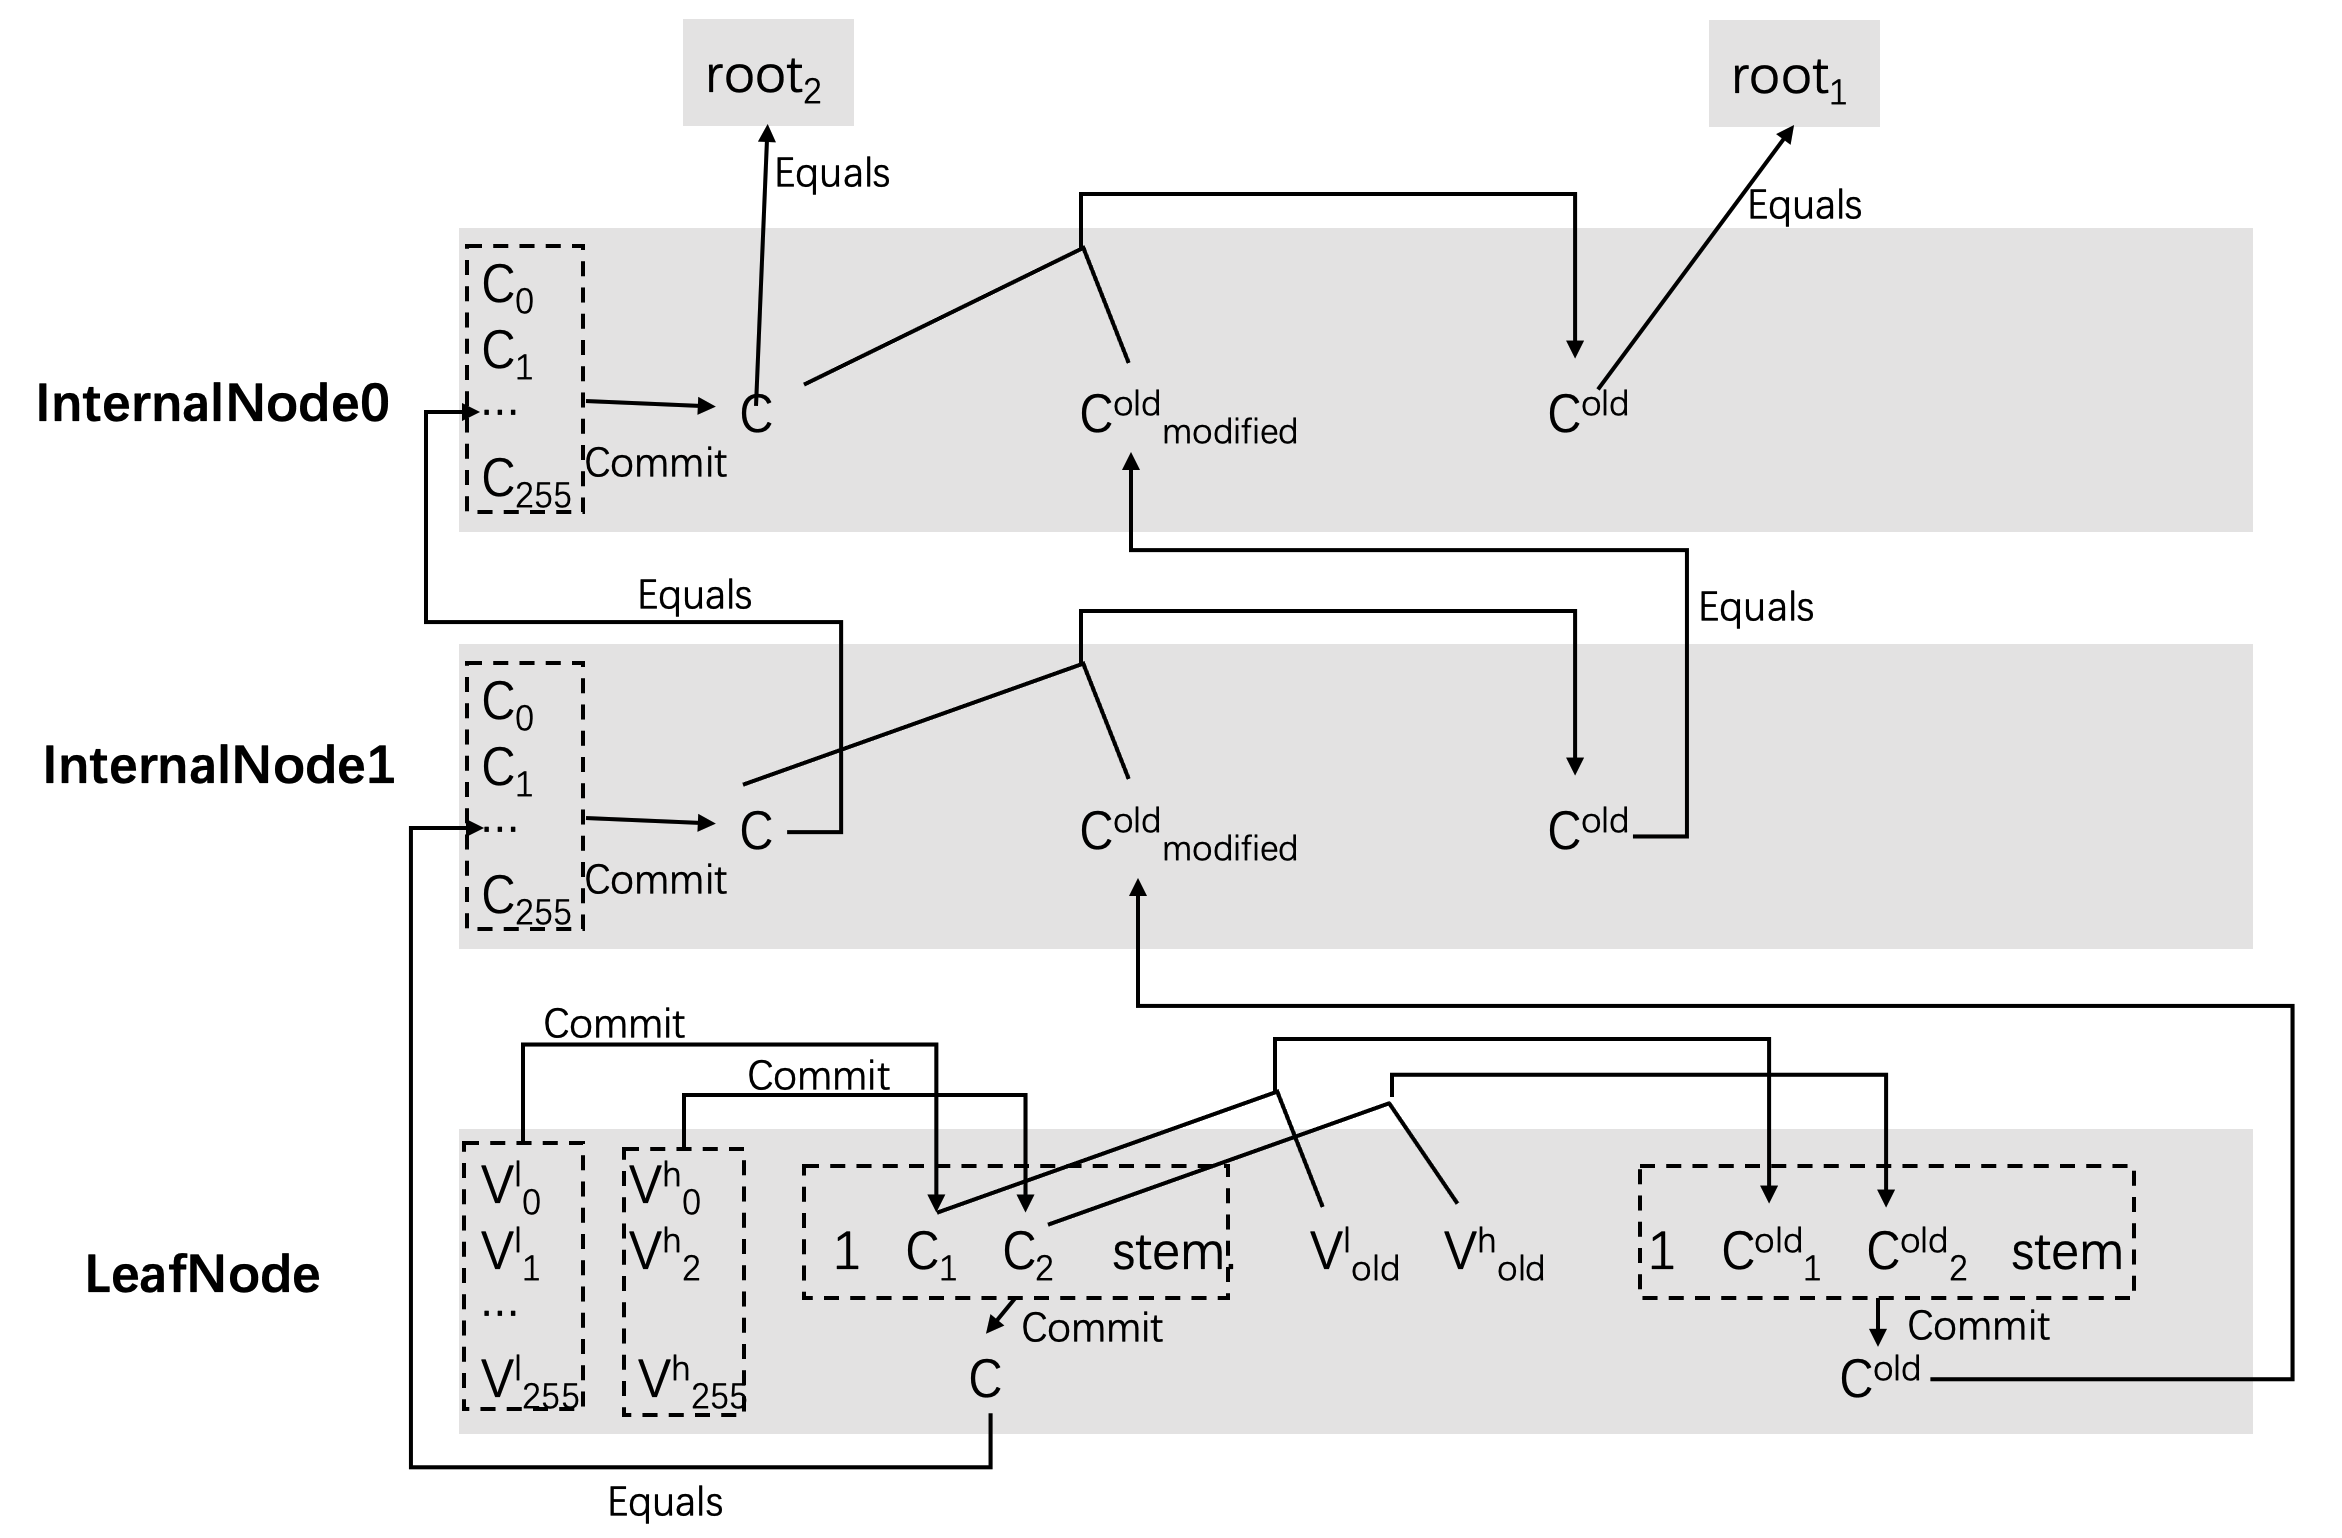
\includegraphics[width=0.8\textwidth]{storage/upgrade_constraint.png}
    \caption{Verkle Tree Update Constraint Schematic}
    \label{fig:upgrade-constraint}
\end{figure}

As for the path related to the updated value, trace table records the completed updated value, i.e.\ $\{V^l_i\}, \{V^h_i\}$ of LeafNode and $\{C_i\}$ of InternalNode. The value before update is represented as $V^l_\text{old}$ and $V^h_\text{old}$ in LeafNode, $C^\text{old}_\text{modified}$ in InternalNode.

In LeafNode, $\{V^l_i\}$ is committed to $C_1$ and $\{V^h_i\}$ is committed to $C_2$. According to the commitment protocol, we can compute the pre-update commitment $C^\text{old}_1$ using $C_1$ and $V^l_\text{old}$, and compute the pre-update commitment $C^\text{old}_2$ using $C_2$ and $V^h_\text{old}$. Finally make a commitment to LeafNode to get the updated commitment $C$ and the commitment before update $C^\text{old}$, and also constrain $C$ to be equal to the commitment of the change line of parent, $C^\text{old}$ to be equal to the pre-change commitment of the change line of parent.

In InternalNode, commit $\{C_i\}$ to $C$, and then the commitment protocol utilizes $C$ and $C^\text{old}_\text{modified}$ to calculate the pre-updated commitment $C^\text{old}$ of this node. Constrain them to be equal to the corresponding values in parent. If the node is on the top-level, constrain $C = \text{root}_2$, $C^\text{old} = \text{root}_1$.

\subsubsection{Constraints for Node Insert}

We have three cases for inserting nodes:
\begin{enumerate}
    \item The node is inserted at the position of EmptyNode in InternalNode.
    \item The node is inserted into the LeafNode position of the InternalNode, and the newly inserted LeafNode has the same stem as the LeafNode at the original position.
    \item The node is inserted into the LeafNode position of the InternalNode, and the newly inserted LeafNode has the different stem from the LeafNode at the original position.
\end{enumerate}

There are no differences between the first/second cases and the constraint logic of node update, which will not be discussed again here. For the third case of inserting a node, the logic of inserting is shown in Figure \ref{fig:insert-constraint-1}.
\begin{figure}[!ht]
    \centering
    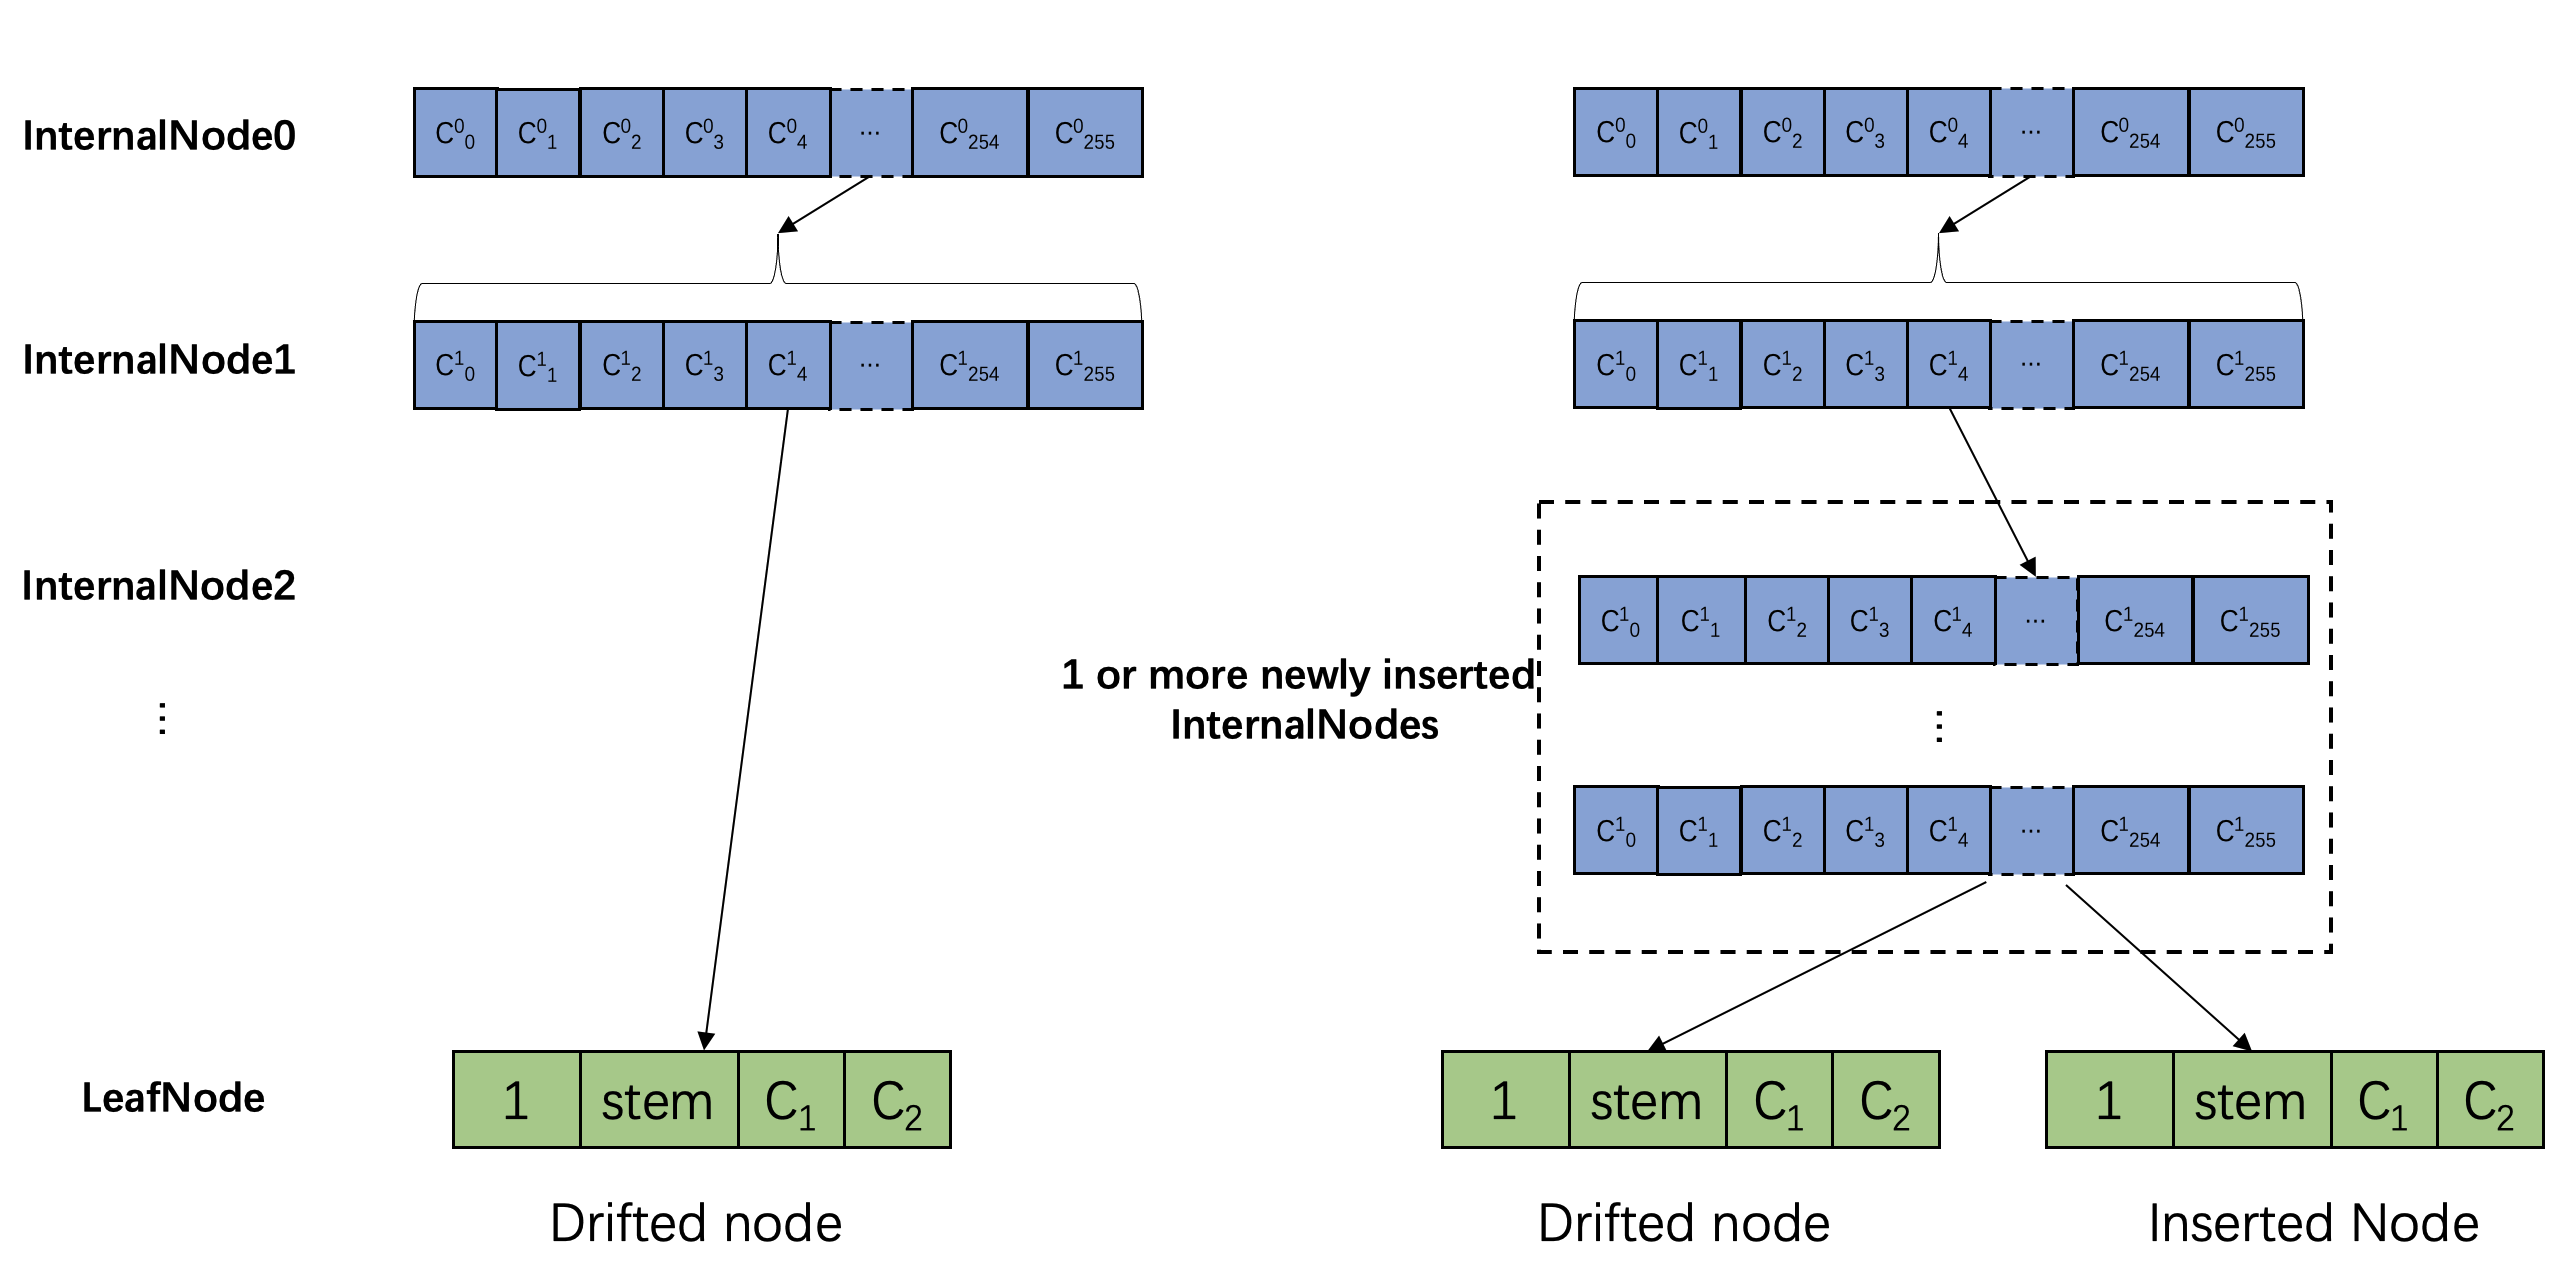
\includegraphics[width=0.8\textwidth]{storage/insert_node1.png}
    \caption{Verkle Tree Update Constraint Schematic}
    \label{fig:insert-constraint-1}
\end{figure}

The position of the newly inserted node in InternalNode has been occupied by a LeafNode, called DriftedNode. Meanwhile, the stem of the newly inserted node is different from that of the original DriftedNode. At this time, one or more InternalNodes need to be added until the paths of the newly inserted LeafNode and the DriftedNode are on different nodes of the InternalNode. Finally, insert the DriftedNode and the newly inserted LeafNode.

In this case, we are supposed to perform constrains to DriftedNode in addition to insert full paths of the node when constraining as Figure \ref{fig:insert-constraint-2}.
\begin{figure}[!ht]
    \centering
    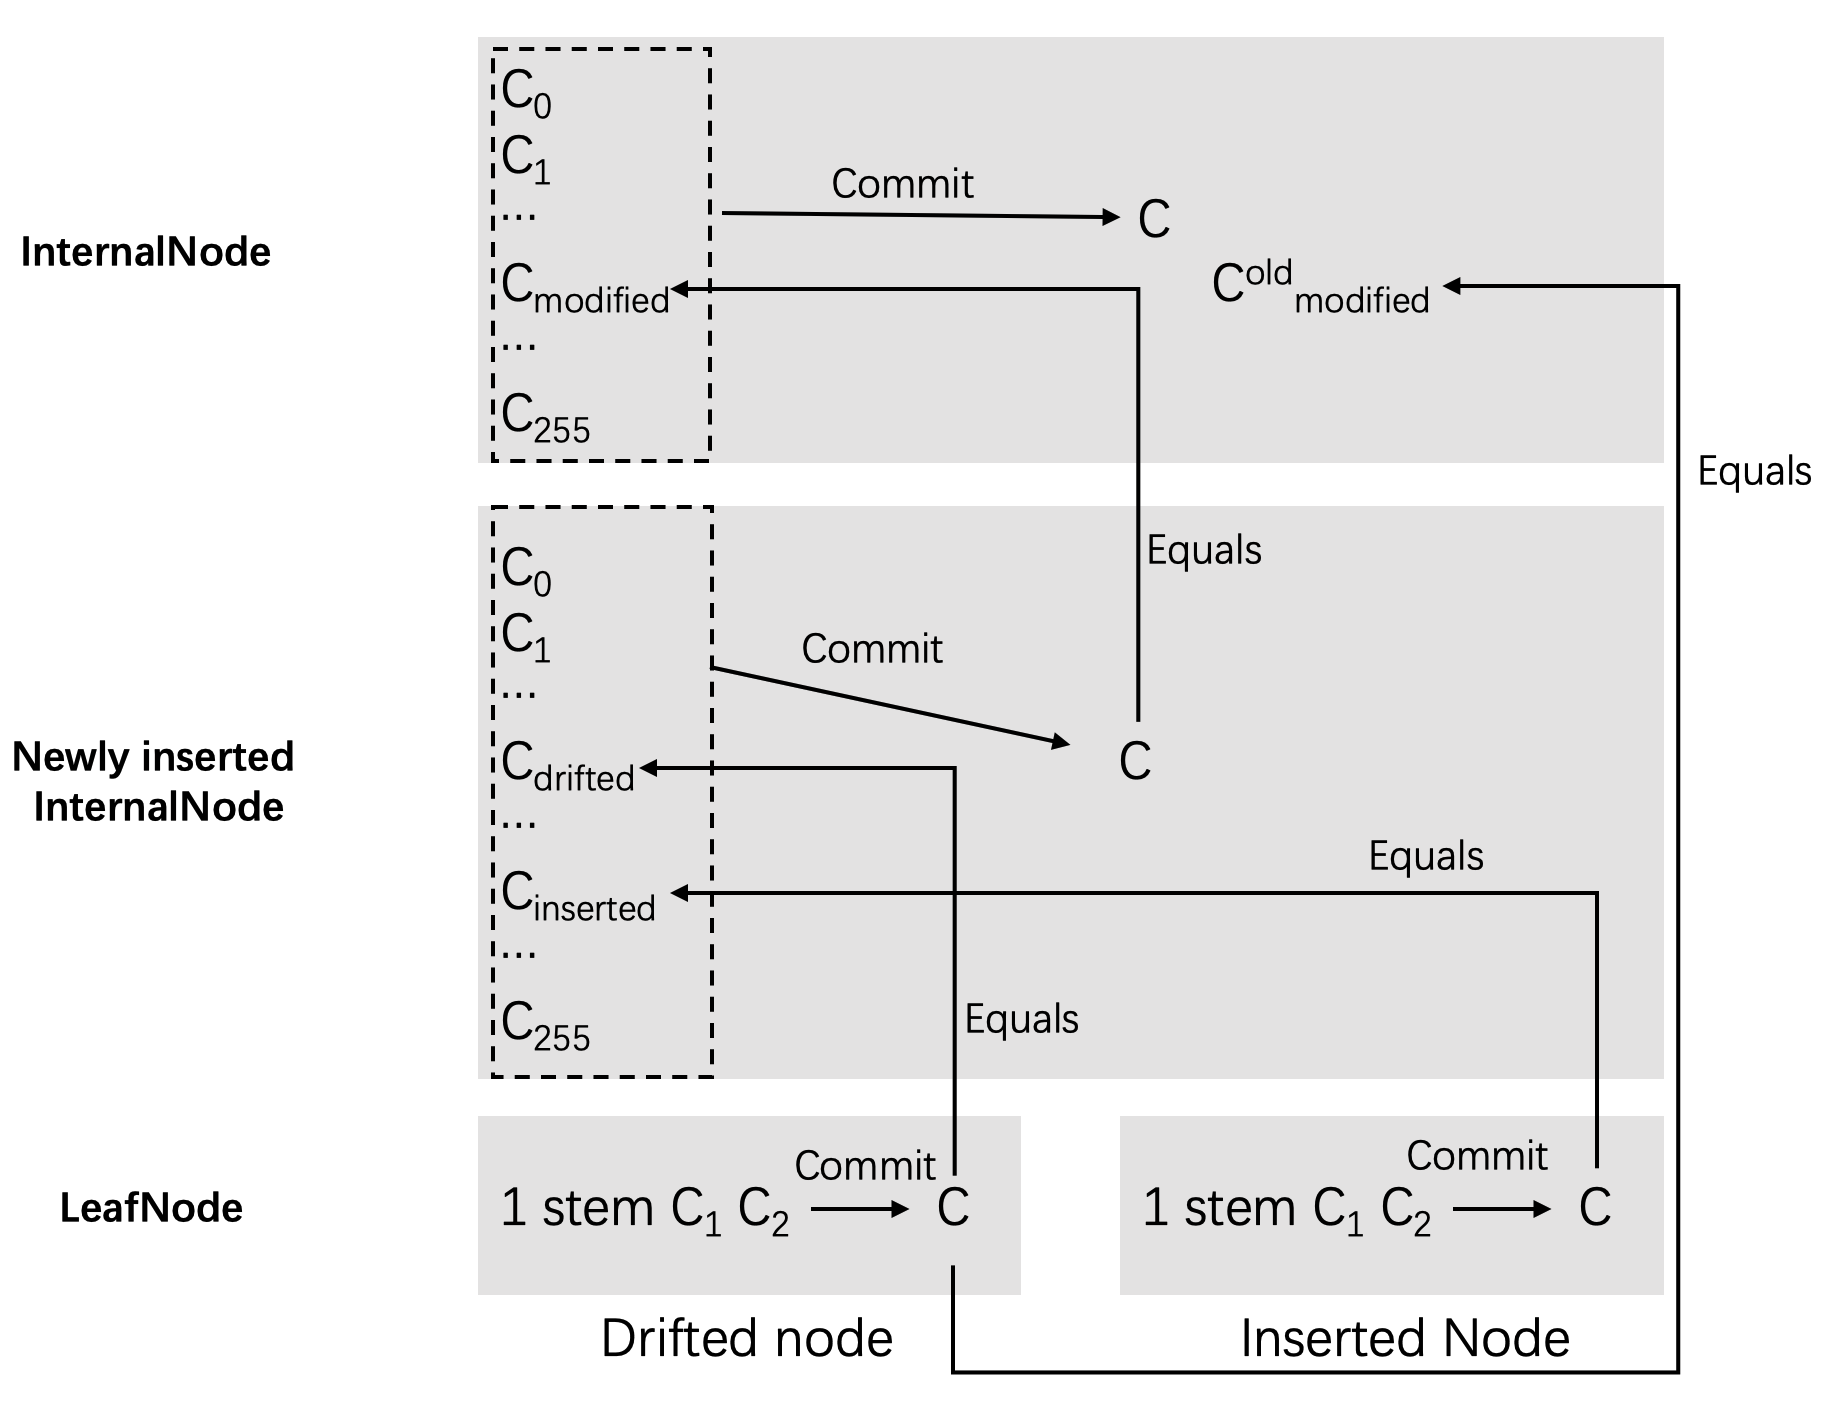
\includegraphics[width=0.8\textwidth]{storage/insert_node2.png}
    \caption{Verkle Tree update constraint schematic}
    \label{fig:insert-constraint-2}
\end{figure}
